%--------------------------------------------------------------------------------------
% Definition of the document
%--------------------------------------------------------------------------------------
\documentclass[12pt]{article}
%--------------------------------------------------------------------------------------
% Define packages needed for the writing
%--------------------------------------------------------------------------------------
% General document formatting
\usepackage[margin=1in]{geometry}
\usepackage[parfill]{parskip}
\usepackage[utf8]{inputenc}    
% Related to math
\usepackage{amsmath,amssymb,amsfonts,amsthm}
% To write derivative more efficiently
\usepackage{physics}
%--------------------------------------------------------------------------------------
% Define the specific setup for the document
%--------------------------------------------------------------------------------------
% Set the font of the equations to Helvetica as well. 
% Increase the spacing between the lines
\linespread{1.5}
%--------------------------------------------------------------------------------------
% THE DOCUMENTS BEGINS
%--------------------------------------------------------------------------------------
\begin{document}
\title{\textbf{New take after rejection from the Bulletin of Mathematical Biology}}
\author{Johannes Borgqvist}
\date{\today}
\maketitle
\tableofcontents
\clearpage
%--------------------------------------------------------------------------------------
% THE INTRO
\section{Introduction}
There are numerous examples of biological systems that give rise to oscillatory behaviour. Some of these are the dynamics of a population consisting of predators and prey, chemical reactions such as the Belusov-Zhabotinskii reaction or the so called Brusselator reaction proposed by Prigogene and Lefever. In these cases, the oscillations have been modelled by mathematical models consisting of a two state system of first order ODEs describing the change in either populations sizes or the concentrations of chemical species over time. Mathematically, these oscillations have been described in terms of linear stability analysis, where the models are firstly linearised around their steady states and then the stability of these local linear systems is determined. However, this analytical tool can merely answer questions about the long term behaviour of the system and it does not reveal what properties that are conserved during these oscillations.

A well-known mathematical technique for deriving conserved properties in theoretical physics is that of symmetry methods. Symmetries are transformations which preserve the defining property of the objects they act on, and in the context of ODEs a symmetry is an operator mapping a solution curve to another solution curve. Moreover, symmetries have been used with huge success in theoretical physics to describe physical entities in terms of conservation laws. Here, we aim to apply these techniques on oscillatory dynamical systems modelled by a two state system of first order ODEs. In particular, we will focus on three models, namely the Lotka-Volterra (LV) model, the SIR model sometimes referred to as the Kermack-McKendrick model, the Belusov-Zhabotinskii (BZ) model and the so called Brusselator. The (dimensionless) LV model is given by 

\begin{equation}
  \begin{split}
    \dv{u}{\tau}&=u(1-v),\\
    \dv{v}{\tau}&=\alpha v(u-1).\\    
    \end{split}
  \label{eq:LV}
\end{equation}
and it describes the ``predator-prey'' dynamics of the evolution of prey $u(\tau)$ and predators $v(\tau)$ at dimensionless time $\tau$. The SIR-model is given by describes the dynamics of the spread of an epidemic in a population consisting of susceptibles $S(t)$, infectives $I(t)$ and the removed class $R(t)$. The model is given by
\begin{equation}
  \begin{split}
    \dv{S}{t}&=-rSI,\\
    \dv{I}{t}&=rSI-aI,\\
    \dv{R}{t}&=aI,\\
    \end{split}
  \label{eq:SIR}
\end{equation}
where $r>0$ is the infection rate and $a>0$ is the removal rate of infectives. Moreover, the BZ model is given by

\begin{equation}
  \begin{split}
    \dv{u}{\tau}&=\dfrac{1}{\varepsilon}v-\dfrac{1}{\varepsilon}\left(\dfrac{1}{3}u^3-u\right),\\
    \dv{v}{\tau}&=-u.\\    
    \end{split}
  \label{eq:BZ}
\end{equation}
describing the formation and degradation of the two chemical species $u(\tau)$ and $v(\tau)$ at time $\tau$. Similarly, another oscillatory chemical system is the so called Brusselator given by

\begin{equation}
  \begin{split}
    \dv{u}{\tau}&=1-(b-1)u+au^2 v,\\
    \dv{v}{\tau}&=bu-au^2 v.\\
    \end{split}
  \label{eq:Brusselator}
\end{equation}
where $u(\tau)$ and $v(\tau)$ are two chemical species. All these three systems can give rise to oscillatory behaviour, and our aim of this work is to be able to characterise oscillations in two state dynamical systems of first order ODEs in terms of their symmetries. Inspired by these three systems, we will restrict our focus to \textit{autonomous} systems, specifically \textit{time-invariant} systems, where the right hand sides are given by polynomials in the states $u$ and $v$. For these type of systems, it is well-known that oscillations correspond to closed trajectories in the $(u,v)$-phase plane and therefore we will furthermore restrict our analysis to symmetries that act exclusively on the $(u,v)$-phase plane meaning that these symmetries are independent of time. Subsequently, we will derive the general equation defining fibre-preserving symmetries restricted to the $(u,v)$-phase plane, after that we will present the symmetries of each of these models and lastly we will interpret their meaning by deriving the differential invariants associated with these symmetries. 



% --------------------------------------------------------------------------------------
%--------------------------------------------------------------------------------------
% LOTKA VOLTERRA
\section{Lotka-Volterra}
We will now consider the symmetries of the LV-model given by
\begin{equation}
  \begin{split}
    \dv{u}{\tau}&=u(1-v),\\
    \dv{v}{\tau}&=\alpha v(u-1).\\    
    \end{split}
  \label{eq:LV}
\end{equation}
Since this model is time-invariant and separable its symmetries are given by
\begin{align}
  X_0&=\partial_\tau+u(1-v)\partial_u+\alpha v(u-1)\partial_v,\label{eq:LV_0}\\
  X_\tau&=\partial_\tau,\label{eq:LV_tau}\\
  X_u&=\dfrac{u}{u-1}\partial_u,\label{eq:LV_u}\\
  X_v&=\dfrac{\alpha v}{1-v}\partial_v.\label{eq:LV_v}
\end{align}
The symmetry of generated by $X_\tau$ in Equation \eqref{eq:LV_tau} corresponds to $\tau$-translations given by
\begin{equation}
\Gamma^{\mathrm{LV},\tau}_{\epsilon}:(\tau,u,v)\mapsto (\tau+\epsilon,u,v).
\end{equation}
For the other two non-trivial generators, i.e. $X_u$ in Equation \eqref{eq:LV_u} and $X_v$ in Equation \eqref{eq:LV_v}, we cannot write down an explicit equation for the symmetry. However, we can write down an implicit expression in terms of their canonical coordinates
\begin{align}
\Gamma^{\mathrm{LV},u}_{\epsilon}:&(s,r_1,r_2)\mapsto(s+\epsilon,r_1,r_2),\quad s=u-\ln(u),r_1=\tau,r_2=v,\label{eq:LV_u}\\
\Gamma^{\mathrm{LV},v}_{\epsilon}:&(s,r_1,r_2)\mapsto(s+\epsilon,r_1,r_2),\quad s=\ln\left(v^{1/\alpha}\right)-\dfrac{v}{\alpha},r_1=\tau,r_2=u.\label{eq:LV_v}\\
\end{align}
In practice, this means that we obtain the transformed coordinates $\hat{u}(\epsilon)$ of $\Gamma^{\mathrm{LV},u}_{\epsilon}$ in Equation \eqref{eq:LV_u} and $\hat{v}(\epsilon)$ of $\Gamma^{\mathrm{LV},v}_{\epsilon}$ in Equation \eqref{eq:LV_v} by solving the following two equations
\begin{align}
u-\ln(u)+\epsilon&=\hat{u}-\ln(\hat{u}),\label{eq:LV_u_implicit}\\
\ln\left(v^{1/\alpha}\right)-\dfrac{v}{\alpha}+\epsilon&=\ln\left(\hat{v}^{1/\alpha}\right)-\dfrac{\hat{v}}{\alpha},\label{eq:LV_v_implicit}
\end{align}
for $\hat{u}$ and $\hat{v}$ respectively. The action of these unidirectional symmetries is illustrated below (Fig \ref{fig:LV_symmetries}). 


\begin{figure}[htbp!]
  \begin{center}
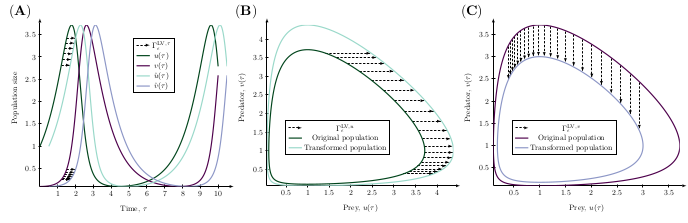
\includegraphics[width=\textwidth]{LV_symmetries}
\caption{\textit{Unidirectional symmetries of the LV-model}. In all cases, the original solution is obtained with the parameter $\alpha=1$, the initial conditions $(u_0,v_0)=(1.00,0.10)$ and the solutions are then transformed with a transformation parameter of $\epsilon=0.5$. (\textbf{A}) The action of the time translation symmetry $\Gamma^{\mathrm{LV},\tau}_{\epsilon}$. (\textbf{B}) The action of the $u$-directional symmetry $\Gamma^{\mathrm{LV},u}_{\epsilon}$. (\textbf{C}) The action of the $v$-directional symmetry $\Gamma^{\mathrm{LV},v}_{\epsilon}$.}
\label{fig:LV_symmetries}
\end{center}
\end{figure}
%--------------------------------------------------------------------------------------
%--------------------------------------------------------------------------------------
% BZ-model
\section{BZ}
The infinitesimal generators of the Lie group that where found with polynomial ans\"atze of degree $d_3=d_4=5$ for the infinitesimals $\eta_1(u,v)$ and $\eta_2(u,v)$ were the following:


\begin{align*}
X_{1}&=\frac{u \left(u^{3} - 3 u - 3 v\right)}{3 e}\partial_u+u^{2}\partial_v,\\
X_{2}&=\frac{v^{2} \left(u^{3} - 3 u - 3 v\right)}{3 e}\partial_u+u v^{2}\partial_v,\\
X_{3}&=\frac{u v \left(u^{3} - 3 u - 3 v\right)}{3 e}\partial_u+u^{2} v\partial_v,\\
X_{4}&=\frac{u^{3} - 3 u - 3 v}{3 e}\partial_u+u\partial_v,\\
X_{5}&=\frac{v \left(u^{3} - 3 u - 3 v\right)}{3 e}\partial_u+u v\partial_v,\\
X_{6}&=\frac{u^{2} \left(u^{3} - 3 u - 3 v\right)}{3 e}\partial_u+u^{3}\partial_v.\\
\end{align*}


Note that the reaction terms are:

\begin{align*}
\omega_1(u,v)&=\frac{v}{e} - \frac{\frac{u^{3}}{3} - u}{e},\\
\omega_2(u,v)&=- u.\\
\end{align*}


so all these generators are trivial.


%--------------------------------------------------------------------------------------
%--------------------------------------------------------------------------------------
% Brusselator
\section{Brusselator}
We remind ourselves that we want to study the Brusselator model

\begin{equation*}
  \begin{split}
    \dv{u}{t}&=1-(b-1)u+au^2 v,\\
    \dv{v}{t}&=bu-au^2 v.\\
    \end{split}
\end{equation*}
and we are looking for a generator of the following kind:
\begin{equation}
X=\xi(t,u,v)\partial_t+\eta_1(t,u,v)\partial_u+\eta_2(t,u,v)\partial_v.
\end{equation}
Now, the first linearised symmetry condition is
\begin{align}
  - a^{2} u^{4} v^{2} \pdv{\xi}{u} + a^{2} u^{4} v^{2} \pdv{\xi}{v} + 2 a b u^{3} v \pdv{\xi}{u} - 2 a b u^{3} v \pdv{\xi}{v}&\nonumber\\
  - 2 a \eta_1 u v - a \eta_2 u^{2} - 2 a u^{3} v \pdv{\xi}{u} + a u^{3} v \pdv{\xi}{v}&\nonumber\\
  + a u^{2} v \pdv{\eta_1}{u} - a u^{2} v \pdv{\eta_1}{v} - 2 a u^{2} v \pdv{\xi}{u} + a u^{2} v \pdv{\xi}{v}&\nonumber\\
  - a u^{2} v \pdv{\xi}{t} - b^{2} u^{2} \pdv{\xi}{u} + b^{2} u^{2} \pdv{\xi}{v} + b \eta_1&\nonumber\\
  + 2 b u^{2} \pdv{\xi}{u} - b u^{2} \pdv{\xi}{v} - b u \pdv{\eta_1}{u} + b u \pdv{\eta_1}{v} &\nonumber\\
  + 2 b u \pdv{\xi}{u} - b u \pdv{\xi}{v} + b u \pdv{\xi}{t} - \eta_1&\nonumber\\
  - u^{2} \pdv{\xi}{u} + u \pdv{\eta_1}{u} - 2 u \pdv{\xi}{u} - u \pdv{\xi}{t} + \pdv{\eta_1}{u}&\nonumber\\
  - \pdv{\xi}{u} + \pdv{\eta_1}{t} - \pdv{\xi}{t}&=0,\label{eq:Brusselator_lin_sym_1}
\end{align}
while the second linearised symmetry condition is given by
\begin{align}
  a^{2} u^{4} v^{2} \pdv{\xi}{u} - a^{2} u^{4} v^{2} \pdv{\xi}{v} - 2 a b u^{3} v \pdv{\xi}{u} + 2 a b u^{3} v \pdv{\xi}{v}&\nonumber\\
  + 2 a \eta_1 u v + a \eta_2 u^{2} + a u^{3} v \pdv{\xi}{u} + a u^{2} v \pdv{\eta_2}{u}&\nonumber\\
  - a u^{2} v \pdv{\eta_2}{v} + a u^{2} v \pdv{\xi}{u} + a u^{2} v \pdv{\xi}{t} + b^{2} u^{2} \pdv{\xi}{u}&\nonumber\\
  - b^{2} u^{2} \pdv{\xi}{v} - b \eta_1 - b u^{2} \pdv{\xi}{u} - b u \pdv{\eta_2}{u}&\nonumber\\
  + b u \pdv{\eta_2}{v} - b u \pdv{\xi}{u} - b u \pdv{\xi}{t} + u \pdv{\eta_2}{u}&\nonumber\\
  + \pdv{\eta_2}{u} + \pdv{\eta_2}{t}&=0.\label{eq:Brusselator_lin_sym_2}
\end{align}


\subsection{Ans\"atze assuming that the equations for the tangents are independent of the states}
Again, the assumption that the derivatives of the tangents are at most functions of the time $t$ amounts to finding the roots of a polynomial of the states $u$ and $v$. Since these monomials are linearly independent we obtain the following equations:
\begin{align}
1:&b \eta_1 - \eta_1 + \pdv{\eta_1}{u} - \pdv{\xi}{u} + \pdv{\eta_1}{t} - \pdv{\xi}{t}=0\\
u:&- b \pdv{\eta_1}{u} + b \pdv{\eta_1}{v} + 2 b \pdv{\xi}{u} - b \pdv{\xi}{v} + b \pdv{\xi}{t} + \pdv{\eta_1}{u} - 2 \pdv{\xi}{u} - \pdv{\xi}{t}=0\\
u v:&- 2 a \eta_1=0\\
u^{2}:&- a \eta_2 - b^{2} \pdv{\xi}{u} + b^{2} \pdv{\xi}{v} + 2 b \pdv{\xi}{u} - b \pdv{\xi}{v} - \pdv{\xi}{u}=0\\
u^{2} v:&a \pdv{\eta_1}{u} - a \pdv{\eta_1}{v} - 2 a \pdv{\xi}{u} + a \pdv{\xi}{v} - a \pdv{\xi}{t}=0\\
u^{3} v:&2 a b \pdv{\xi}{u} - 2 a b \pdv{\xi}{v} - 2 a \pdv{\xi}{u} + a \pdv{\xi}{v}=0\\
u^{4} v^{2}:&- a^{2} \pdv{\xi}{u} + a^{2} \pdv{\xi}{v}=0,
\end{align}
for the first linearised symmetry condition and the following equations
\begin{align}
1:&- b \eta_1 + \pdv{\eta_2}{u} + \pdv{\eta_2}{t}=0\\
u:&- b \pdv{\eta_2}{u} + b \pdv{\eta_2}{v} - b \pdv{\xi}{u} - b \pdv{\xi}{t} + \pdv{\eta_2}{u}=0\\
u v:&2 a \eta_1=0\\
u^{2}:&a \eta_2 + b^{2} \pdv{\xi}{u} - b^{2} \pdv{\xi}{v} - b \pdv{\xi}{u}=0\\
u^{2} v:&a \pdv{\eta_2}{u} - a \pdv{\eta_2}{v} + a \pdv{\xi}{u} + a \pdv{\xi}{t}=0\\
u^{3} v:&- 2 a b \pdv{\xi}{u} + 2 a b \pdv{\xi}{v} + a \pdv{\xi}{u}=0\\
u^{4} v^{2}:&a^{2} \pdv{\xi}{u} - a^{2} \pdv{\xi}{v}=0,
\end{align}
for the second linearised symmetry condition.
%--------------------------------------------------------------------------------------
%--------------------------------------------------------------------------------------
% THE DOCUMENT ENDS
%--------------------------------------------------------------------------------------
\end{document}